% Kommentare für den Editor (TexWorks/TexMakerX)
% !TeX encoding   = utf8
% !TeX spellcheck = de-DE

% --- LaTeX Vorlage ------------------------------------------------------
% speziell für einfache Dokumente wie Praktikumsprotokolle
%
% Autor: Matthias Pospiech (matthias@pospiech.eu)
% ------------------------------------------------------------------------

% Dokumentenklasse (Koma Script) -----------------------------------------
\documentclass[%
   %draft,     % Entwurfsstadium
   final,      % fertiges Dokument
   paper=a4, paper=portrait, pagesize=auto, % Papier Einstellungen
   fontsize=11pt, % Schriftgröße
   ngerman, % Sprache 
 ]{scrartcl} % Classes: scrartcl, scrreprt, scrbook

% ~~~~~~~~~~~~~~~~~~~~~~~~~~~~~~~~~~~~~~~~~~~~~~~~~~~~~~~~~~~~~~~~~~~~~~~~
% encoding
% ~~~~~~~~~~~~~~~~~~~~~~~~~~~~~~~~~~~~~~~~~~~~~~~~~~~~~~~~~~~~~~~~~~~~~~~~

% Encoding der Dateien (sonst funktionieren Umlaute nicht)
\usepackage[utf8]{inputenc}
\setlength\parindent{0pt} % Removes all indentation from paragraphs
\usepackage{listings}

\usepackage{tabularx}


\newcommand{\margin}{-0.5cm}
\newenvironment{changemargin}[2]{%
	\begin{list}{}{%
			\setlength{\topsep}{0pt}%
			\setlength{\leftmargin}{#1}%
			\setlength{\rightmargin}{#2}%
			\setlength{\listparindent}{\parindent}%
			\setlength{\itemindent}{\parindent}%
			\setlength{\parsep}{\parskip}%
		}%
		\item[]}{\end{list}}

% Encoding der Verzeichnisse (für Pfade mit Umlauten und Leerzeichne)
\usepackage[%
   extendedchars, encoding, multidot, space,
   filenameencoding=latin1, % Windows XP, Vista, 7
   % filenameencoding=utf8,   % Linux, OS X
]{grffile}

% ~~~~~~~~~~~~~~~~~~~~~~~~~~~~~~~~~~~~~~~~~~~~~~~~~~~~~~~~~~~~~~~~~~~~~~~~
% Pakete und Stile
% ~~~~~~~~~~~~~~~~~~~~~~~~~~~~~~~~~~~~~~~~~~~~~~~~~~~~~~~~~~~~~~~~~~~~~~~~
% Schriften
\input{preambel/fonts}
% Pakete Laden
% ~~~~~~~~~~~~~~~~~~~~~~~~~~~~~~~~~~~~~~~~~~~~~~~~~~~~~~~~~~~~~~~~~~~~~~~~
% These packages must be loaded before all others
% (primarily because they are required by other packages)
% ~~~~~~~~~~~~~~~~~~~~~~~~~~~~~~~~~~~~~~~~~~~~~~~~~~~~~~~~~~~~~~~~~~~~~~~~
\usepackage{calc}
\usepackage{fixltx2e}	% Fix known LaTeX2e bugs

\usepackage[english]{babel} 			% Sprache
\usepackage[dvipsnames, table]{xcolor} 	% Farben

% ~~~~~~~~~~~~~~~~~~~~~~~~~~~~~~~~~~~~~~~~~~~~~~~~~~~~~~~~~~~~~~~~~~~~~~~~
% Hinzugefuegt bei mir (marvin)
% ~~~~~~~~~~~~~~~~~~~~~~~~~~~~~~~~~~~~~~~~~~~~~~~~~~~~~~~~~~~~~~~~~~~~~~~~


% ~~~~~~~~~~~~~~~~~~~~~~~~~~~~~~~~~~~~~~~~~~~~~~~~~~~~~~~~~~~~~~~~~~~~~~~~
% Bilder, Gleitumgebungen und Platzierung
% ~~~~~~~~~~~~~~~~~~~~~~~~~~~~~~~~~~~~~~~~~~~~~~~~~~~~~~~~~~~~~~~~~~~~~~~~

\usepackage[]{graphicx}					% Graphiken
\usepackage{epstopdf}		% konvertiert eps in pdf

% provides new floats and enables H float modifier option
\usepackage{float}
% Floats immer erst nach der Referenz setzen
\usepackage{flafter}
% Alel Floats werden vor der nächsten section ausgegeben
\usepackage[section]{placeins} 
%

% ~~~~~~~~~~~~~~~~~~~~~~~~~~~~~~~~~~~~~~~~~~~~~~~~~~~~~~~~~~~~~~~~~~~~~~~~
% Beschriftungen (captions)
% ~~~~~~~~~~~~~~~~~~~~~~~~~~~~~~~~~~~~~~~~~~~~~~~~~~~~~~~~~~~~~~~~~~~~~~~~

\usepackage{caption}
\usepackage{subcaption}

% ~~~~~~~~~~~~~~~~~~~~~~~~~~~~~~~~~~~~~~~~~~~~~~~~~~~~~~~~~~~~~~~~~~~~~~~~
% Math
% ~~~~~~~~~~~~~~~~~~~~~~~~~~~~~~~~~~~~~~~~~~~~~~~~~~~~~~~~~~~~~~~~~~~~~~~~

% Base Math Package
\usepackage[fleqn]{amsmath} 
% Warnt bei Benutzung von Befehlen die mit amsmath inkompatibel sind.
\usepackage[all, error]{onlyamsmath}

% ~~~~~~~~~~~~~~~~~~~~~~~~~~~~~~~~~~~~~~~~~~~~~~~~~~~~~~~~~~~~~~~~~~~~~~~~
% Science
% ~~~~~~~~~~~~~~~~~~~~~~~~~~~~~~~~~~~~~~~~~~~~~~~~~~~~~~~~~~~~~~~~~~~~~~~~

% Einheiten und Zahlenformatierung
\usepackage{siunitx}

% ~~~~~~~~~~~~~~~~~~~~~~~~~~~~~~~~~~~~~~~~~~~~~~~~~~~~~~~~~~~~~~~~~~~~~~~~
% Tables (Tabular)
% ~~~~~~~~~~~~~~~~~~~~~~~~~~~~~~~~~~~~~~~~~~~~~~~~~~~~~~~~~~~~~~~~~~~~~~~~

\usepackage{booktabs}
\usepackage{ltxtable} % Longtable + tabularx

% ~~~~~~~~~~~~~~~~~~~~~~~~~~~~~~~~~~~~~~~~~~~~~~~~~~~~~~~~~~~~~~~~~~~~~~~~
% text related packages
% ~~~~~~~~~~~~~~~~~~~~~~~~~~~~~~~~~~~~~~~~~~~~~~~~~~~~~~~~~~~~~~~~~~~~~~~~

\usepackage{url}            % Befehl \url{...}
\usepackage{enumitem}		% Kompakte Listen

% Neue Befehle: \Centering, \RaggedLeft, and \RaggedRight, ... 
\usepackage{ragged2e}


% ~~~~~~~~~~~~~~~~~~~~~~~~~~~~~~~~~~~~~~~~~~~~~~~~~~~~~~~~~~~~~~~~~~~~~~~~
% Citations
% ~~~~~~~~~~~~~~~~~~~~~~~~~~~~~~~~~~~~~~~~~~~~~~~~~~~~~~~~~~~~~~~~~~~~~~~~
%\usepackage[
%	style=alphabetic, % Loads the bibliography and the citation style 
%	natbib=true, % define natbib compatible cite commands
%]{biblatex}	
% Other options:
%	style=numeric, % 
%	style=numeric-comp,    % [1–3, 7, 8]
%	style=numeric-verb,    % [2]; [5]; [6]


% ~~~~~~~~~~~~~~~~~~~~~~~~~~~~~~~~~~~~~~~~~~~~~~~~~~~~~~~~~~~~~~~~~~~~~~~~
% layout packages
% ~~~~~~~~~~~~~~~~~~~~~~~~~~~~~~~~~~~~~~~~~~~~~~~~~~~~~~~~~~~~~~~~~~~~~~~~
%
% Befehle für 1,5 und 2 zeilig: 
% \singlespacing, \onehalfspacing und \doublespacing
\usepackage{setspace}

% ~~~~~~~~~~~~~~~~~~~~~~~~~~~~~~~~~~~~~~~~~~~~~~~~~~~~~~~~~~~~~~~~~~~~~~~~
% Kopf und Fusszeile
% ~~~~~~~~~~~~~~~~~~~~~~~~~~~~~~~~~~~~~~~~~~~~~~~~~~~~~~~~~~~~~~~~~~~~~~~~

% Kopf und Fusszeile mit scrpage2 einstellen
\usepackage[automark, komastyle, nouppercase]{scrpage2}

% ~~~~~~~~~~~~~~~~~~~~~~~~~~~~~~~~~~~~~~~~~~~~~~~~~~~~~~~~~~~~~~~~~~~~~~~~
% pdf packages
% ~~~~~~~~~~~~~~~~~~~~~~~~~~~~~~~~~~~~~~~~~~~~~~~~~~~~~~~~~~~~~~~~~~~~~~~~

% Include pages from external PDF documents in LaTeX documents
\usepackage{pdfpages} 

% Optischer Randausgleich mit pdfTeX
\usepackage{microtype}

% Links
\usepackage[hidelinks]{hyperref}

% Einstellungen und Layoutstile 
\input{preambel/style}


% ~~~~~~~~~~~~~~~~~~~~~~~~~~~~~~~~~~~~~~~~~~~~~~~~~~~~~~~~~~~~~~~~~~~~~~~~
% Eigene Befehle
% ~~~~~~~~~~~~~~~~~~~~~~~~~~~~~~~~~~~~~~~~~~~~~~~~~~~~~~~~~~~~~~~~~~~~~~~~
\input{macros/newcommands}


\usepackage{listings}
\usepackage{color}

% color definitions and code style
\definecolor{codeblue}{RGB}{58,33,158}
\definecolor{codegreen}{rgb}{0,0.47,0}
\definecolor{codegray}{rgb}{0.5,0.5,0.5}
\definecolor{codepurple}{rgb}{0.55,0,0.53}
\definecolor{backcolour}{rgb}{0.97,0.97,0.97}

\lstdefinestyle{vhdlstyle}{
	basicstyle=\small,
	backgroundcolor=\color{backcolour},
	commentstyle=\color{deepred},
	keywordstyle=\color{codepurple},
	numberstyle=\tiny\color{codegray},
	stringstyle=\color{codegreen},
	breakatwhitespace=false,         
	breaklines=true,                 
	captionpos=b,                    
	keepspaces=true,                
	showspaces=false,                
	showstringspaces=false,
	showtabs=false,                  
	tabsize=2,
	emphstyle=\color{codeblue},
	frame=single,
	captionpos=t,
	% language specific
	language=vhdl,
	otherkeywords={},
	emph={}
}

\lstdefinestyle{cppstyle}{
	basicstyle=\small,
	backgroundcolor=\color{backcolour},
	commentstyle=\color{deepred},
	keywordstyle=\color{codepurple},
	numberstyle=\tiny\color{codegray},
	stringstyle=\color{codegreen},
	breakatwhitespace=false,         
	breaklines=true,                 
	captionpos=b,                    
	keepspaces=true,                
	showspaces=false,                
	showstringspaces=false,
	showtabs=false,                  
	tabsize=2,
	emphstyle=\color{codeblue},
	frame=single,
	captionpos=t,
	% language specific
	language=c++,
	otherkeywords={TEST_CASE,SECTION,REQUIRE,;,\{,\},+,-,*,/},
	emph={std}
}

\lstdefinestyle{pythonstyle}{
	basicstyle=\small,
	backgroundcolor=\color{backcolour},
	commentstyle=\color{deepred},
	keywordstyle=\color{codepurple},
	numberstyle=\tiny\color{codegray},
	stringstyle=\color{codegreen},
	breakatwhitespace=false,         
	breaklines=true,                 
	captionpos=b,                    
	keepspaces=true,                
	showspaces=false,                
	showstringspaces=false,
	showtabs=false,                  
	tabsize=2,
	emphstyle=\color{codeblue},
	frame=single,
	captionpos=t,
	% language specific
	language=Python,
	otherkeywords={},
	emph={}
}

% VHDL environment
\lstnewenvironment{vhdl} {
	\lstset{style=vhdlstyle}
}{}

% Python environment
\lstnewenvironment{python} {
	\lstset{style=pythonstyle}
}{}
%c++ environment
\lstnewenvironment{cpp} {
	\lstset{style=cppstyle}
}{}

% ~~~~~~~~~~~~~~~~~~~~~~~~~~~~~~~~~~~~~~~~~~~~~~~~~~~~~~~~~~~~~~~~~~~~~~~~
% Eigene Befehle
% ~~~~~~~~~~~~~~~~~~~~~~~~~~~~~~~~~~~~~~~~~~~~~~~~~~~~~~~~~~~~~~~~~~~~~~~~
\input{content/Silbentrennung}

\listfiles % schreibt alle verwendeten Dateien in die log Datei


% custom fonts and math extensions
\usepackage{fontspec}
\usepackage{unicode-math} 
\usepackage{amsmath}                % Für fancy Formel-Umgebungen.
\usepackage{amssymb}                % Für fancy Mathe-Zeichen.
\usepackage{amsfonts}               % Für fancy Mathe-Schrift im math mode (Cambria Math)
\usepackage{siunitx}

\newfontfamily{\amethysta}{Amethysta-Regular}
[Path = fonts/amethysta/, Extension = .ttf]
\DeclareTextFontCommand{\textdedication}{\amethysta}

%\newfontfamily{\computermodern}{cmunrm}
%[Path = fonts/computer-modern/, Extension = .ttf]
%\DeclareTextFontCommand{\textdedication}{\computermodern}

\usepackage{pifont}
\newcommand{\cmark}{\ding{51}}%
\newcommand{\xmark}{\ding{55}}%

\newfontfamily{\polyglott}{polyglott}
[Path = fonts/polyglott/, Extension = .ttf]
\DeclareTextFontCommand{\textdedication}{\polyglott}

\setmainfont[Path = fonts/amethysta/, Extension = .ttf]{Amethysta-Regular}
%\setmainfont[Path = fonts/cormorant/, Extension = .ttf]{Cormorant-Regular}
\setmathfont{Cambria Math}

% select toc font
\usepackage{tocloft,lipsum,pgffor,sectsty}

\setcounter{tocdepth}{2}% Include up to \subsection in ToC

% Font changes to ToC content of sectional units
\renewcommand{\cftpartfont}{\polyglott\bfseries}% \part font in ToC
\renewcommand{\cftsecfont}{\normalfont\sffamily\large\bfseries}           % \section font in ToC
\renewcommand{\cftsubsecfont}{\normalfont\sffamily\large}        % \subsection font in ToC
%\renewcommand{\cftsubsubsecfont}{\polyglott\small}       % \subsubsection font in ToC

% Font changes to document content of sectional units
\renewcommand{\partfont}{\normalfont\sffamily\Huge\bfseries}
\renewcommand{\sectionfont}{\normalfont\sffamily\Huge\bfseries}

\usepackage{titlesec}

\titleformat*{\section}{\sffamily\LARGE\bfseries}
\titleformat*{\subsection}{\sffamily\Large\bfseries}
\titleformat*{\subsubsection}{\sffamily\large\bfseries}
\titleformat*{\paragraph}{\sffamily\large\bfseries}
\titleformat*{\subparagraph}{\sffamily\large\bfseries}

%% Dokument Beginn %%%%%%%%%%%%%%%%%%%%%%%%%%%%%%%%%%%%%%%%%%%%%%%%%%%%%%%%
\begin{document}	

\graphicspath{{content/figures/}} % Location of the graphics files {{}} because of windows

% Automatische Titelseite

\title{General Purpose Control GUI for tabletop lab devices and more}
\author{Marvin Peter}
\date{\today}
\maketitle
\begin{figure}[h]
	\centering
	\includegraphics[scale=0.5]{content/figures/jlu-logo.ps}
\end{figure}
\thispagestyle{empty}
\newpage
{\tableofcontents}
\thispagestyle{empty}
\newcommand{\env}[1]{\texttt{#1}}
\newcommand{\command}[1]{\texttt{#1}}
\newcommand{\package}[1]{\texttt{\itshape#1}}
\newcommand{\engl}[1]{(engl: \textit{#1})\xspace}
\newpage

\setcounter{page}{1}
\automark[section]{subsection}
\clearscrheadings
\ihead{\headmark}
\ohead{\pagemark} 
\pagestyle{scrheadings} 
\setheadsepline{.5pt}
% Testdokumente (auskommentieren!)

%\input{content/demo/demo.tex}
%\input{content/demo/latexexample.tex}

% in diese Datei gehört der Inhalt des Dokumentes:
\newpage
\section{Introduction}
This manual should give you an insight into the general purpose control software.
This software is intended to be used as control software for all kinds of lab measurement devices and generally all devices that can be connected by some kind of serial interface (e.g. uart, spi or i2c). The main focus is on lab devices that use the scpi protocol standard for messages which uses plain text over uart (via RS232) to transmit data. As stop character usually a linefeed, carriage return or both are being used. Not all lab devices use this standard and not all which use the standard are consistent in their usage. Specific commands vary a lot so there is a class for each device that translates the specific commands from hardware level to the abstract form that the readout program understands. More about this later. \par\bigskip

Here a list about which devices are already thought of or are already \\supported/implemented:\\
(exists means there is already a child class for this device)

\begin{center}
\polyglott
\rowcolors{2}{gray!10}{white}
\begin{tabularx}{\textwidth}{|X|c|c|c|c|}
\rowcolor{gray!20}
\hline
device name & conn. type & exists & works partially & complete \\
\hline
Keithley 2000 & uart (scpi) & \cmark & \cmark & \\
Keithley 2410 & uart (scpi) & \cmark & \cmark & \\
Rigol DSA1030A &  & \cmark & & \\
Sourcetronic ST2819A &  & \cmark & & \\
Tektronix DMM4020 &  & \cmark & & \\
Voltcraft PSP1803 &  & \cmark & & \\
HP 34401A & & \cmark & & \\
Hameg HM8143 & & \cmark & & \\
GW Instek GPD4303S & & \cmark & & \\
\hline
Adafruit ssd1306 & i2c & & & \\
ADS1115 & i2c & & & \\

BME280 & i2c & & & \\
BMP180 & i2c & & & \\
EEPROM24AA02 & i2c & & & \\
HMC5883 & i2c & & & \\
LM75 & i2c & & & \\

MCP4728 & i2c & & & \\
PCA9536 & i2c & & & \\
SHT21 & i2c & & & \\
SHT31 & i2c & & & \\
TCA9546A & i2c & & & \\
X9119 & i2c & & & \\
\hline
TDC7200 & spi & & & \\
GPX2 & spi & & & \\
\hline
\end{tabularx}
\end{center}
\newpage
\section{Classes and program functionality overview}
The GUI application is written in QT (c++). It contains of a main window which holds different kinds of widgets that can be dragged around. It also features a settings dialogue and a serial console for manually sending messages.
A class diagram can be seen in figure~\ref{fig:classdiagram}.
\par\bigskip
\begin{figure}[h]
	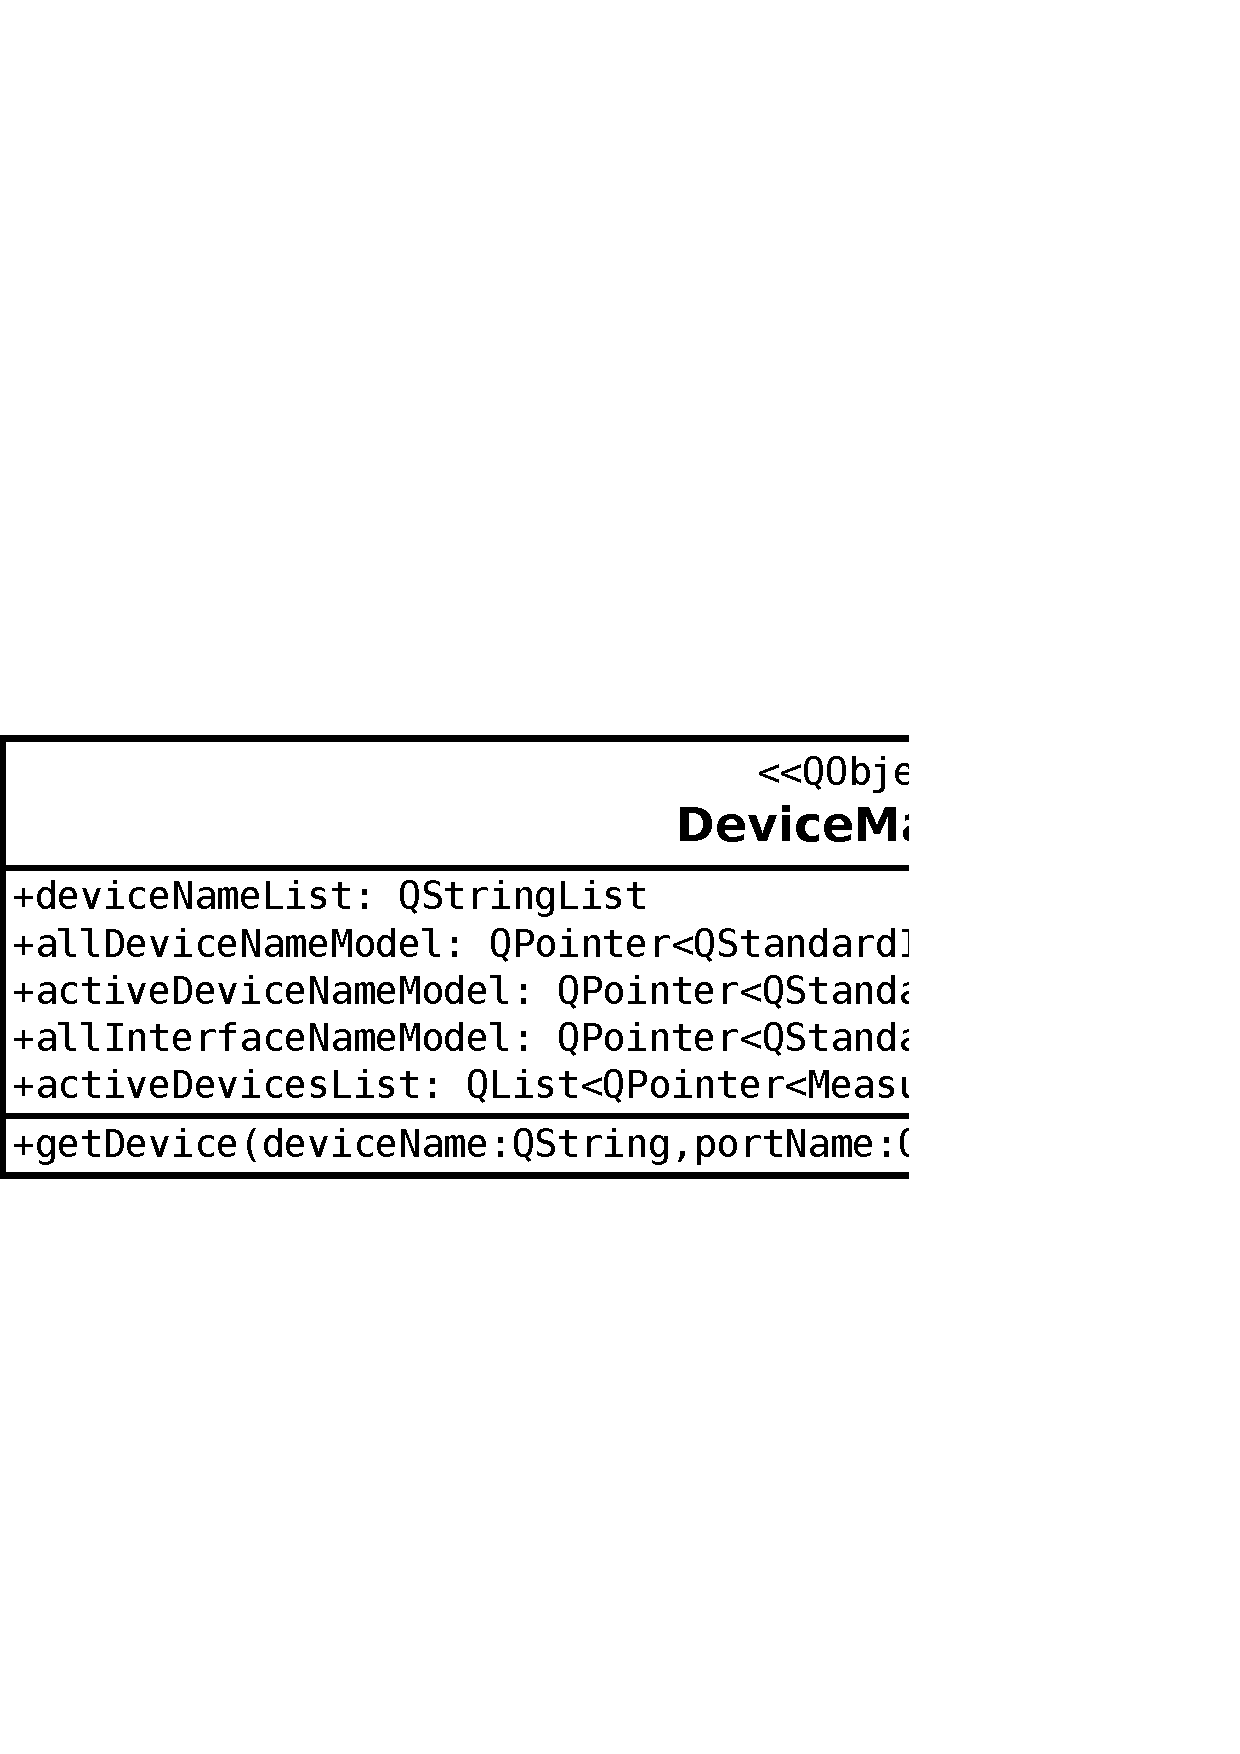
\includegraphics[width=\textwidth]{generalpurposecontrol.png}
	\caption{class diagram}
	\label{fig:classdiagram}
\end{figure}
\par\bigskip

The MainWindow class can contain objects of type MeasurementDevice and ScanParameterSelection in different areas of the GUI as can be seen in figure~\ref{fig:guicolored}.\par\bigskip

The MeasurementDevice is for itself a widget that has a graphical representation of the parameters one hardware device might have: a device name, port (address) and a table of values that can be written or read by the device, for example voltage or current. Also the information of read/write access possibility is in this table. MeasurementDevice has abstract functions for starting measurements and sending the results to some other class and is therefore the parent class of all device classes. Polymorphism is used to store all different child classes inside the same layout in the main window.\par\bigskip

The ScanParameterSelection class is used to set write-enabled parameters to certain values or ramping them during a measurement. A previously instantiated device can be selected from the drop down menu in ScanParameterSelection thanks to the DeviceManager class which holds an overview of all instantiated device objects and providing the item models for the drop down menus etc.\par\bigskip

When a measurement is started in the main window by clicking 'start measurement' all ScanParameterSelection widgets create basically a nested loop. At each measurement step only one ramping parameter will be changed, allowing ramping of multiple parameters on multiple devices controlled by only one application. The progress of the whole measurement procedure is tracked by a progress bar which is calculated at each increment, showing the overall progress.\newpage

\begin{figure}[h]
	\includegraphics[width=\textwidth]{gui_all_colored.png}
	\caption{\\
		\color{Red}red\color{black}: Device selection area;\\
		\color{Green}green\color{black}: Scan parameter selection area;\\
		\color{Blue}blue\color{black}: Serial console pop-up dialog; \\
		\color{Purple}purple\color{black}: measurement / time selection and info area}
	\label{fig:guicolored}
\end{figure}
\par\bigskip


\section{Create new device class}
\subsection{Add class to DeviceManager getDevice function}
Make sure that the getDevice function returns the correct newly created MeasurementDevice subclass.
\lstinputlisting[style=cppstyle]{content/code/devicemanager.cpp}
\newpage
\appendix
\section{Sources}
%\lstinputlisting[style=cppstyle]{content/code/main.cpp}
\begin{cpp}
	#include "mainwindow.h"
	#include <QApplication>
	
	int main(int argc, char *argv[])
	{
		QApplication a(argc, argv);
		MainWindow w;
		w.show();
		
		return a.exec();
	}
\end{cpp}
\end{document}
%% Dokument ENDE %%%%%%%%%%%%%%%%%%%%%%%%%%%%%%%%%%%%%%%%%%%%%%%%%%%%%%%%%%

